\documentclass{homework}

\usepackage{graphicx}
\usepackage{minted}
\usepackage{xspace}


\newcommand{\kat}{Kathará\xspace}
\newcommand{\opn}{OPNsense\xspace}
\newcommand{\vb}{VirtualBox\xspace}

\newcommand{\client}{\textit{client}\xspace}
\newcommand{\dmz}{\textit{DMZ}\xspace}
\newcommand{\ser}{\textit{internal server}\xspace}
\newcommand{\intfw}{\textit{intfw}\xspace}
\newcommand{\mainfw}{\textit{mainfw}\xspace}

\newcommand{\lan}{\textit{LAN}\xspace}
\newcommand{\opt}{\textit{OPT1}\xspace}
\newcommand{\wan}{\textit{WAN}\xspace}


\title{Practical Network Defense - Lab 5}
\author{Alessandro Serpi - 1647244}
\date{29 March 2019}


\begin{document}
    \maketitle
    \tableofcontents
    
    
    \pagebreak
    \section{Introduction}
    In this assignment we have to set up two VPNs: one for road warriors (people who work outside the office and travel for business) and another between the two firewall.
    The assignment has been carried out on a local environment, please refer to the previous report for the network topology and configuration.
    
    \section{VPN for the road warriors}
    \subsection{Users}
    \vspace{-10pt}
    \begin{figure}[H]
        \centering
        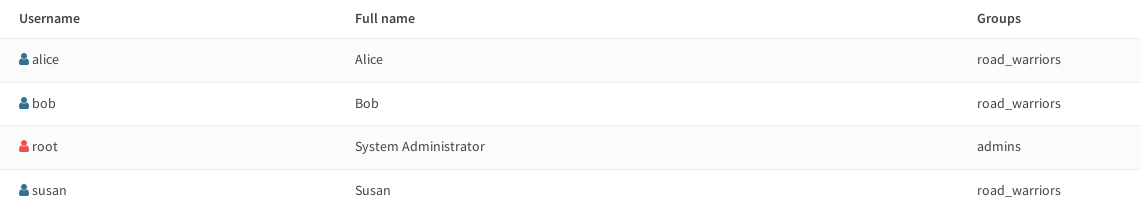
\includegraphics[width=\linewidth]{openvpn/users}
        \label{fig:users}
    \end{figure}
    \vspace{-20pt}
    Create the three new users \textit{alice}, \textit{bob} and \textit{susan} in System $\rightarrow$ Access $\rightarrow$ Users.
    All fields except username and password are optional and may be omitted. 
    Then, create the group \textit{road\_warriors} and add to it the newly created users.
    
    \subsection{Server}
    Create a new server in VPN $\rightarrow$ OpenVPN $\rightarrow$ Servers and populate it with the following options.
    The encryption settings provide additional security with respect to the default (except for the password-only authentication mode, which has been decided with smartphones in mind), while the subnet \texttt{10.10.0.0/24} has been chosen without a precise reason.
    \begin{figure}[H]
        \centering
        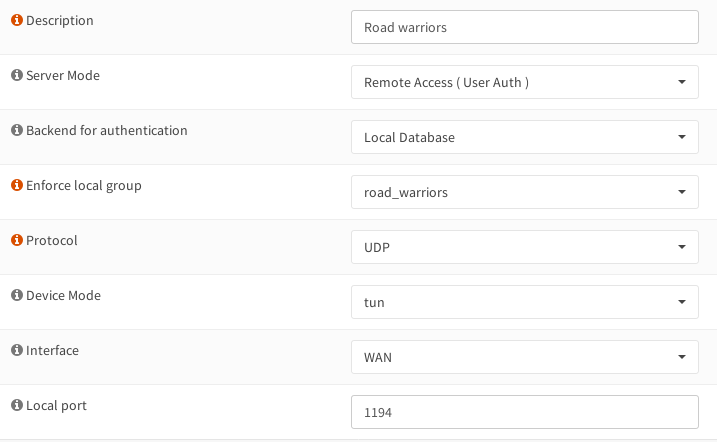
\includegraphics[width=\linewidth]{openvpn/settings-general}
        \label{fig:openvpn-settings-general}
    \end{figure}
    \vspace{-20pt}
    \begin{figure}[H]
        \centering
        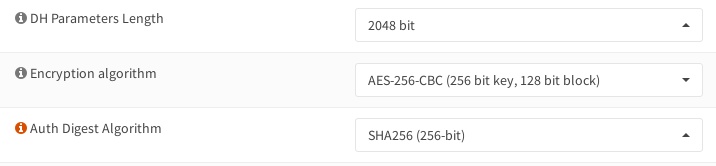
\includegraphics[width=\linewidth]{openvpn/settings-security}
        \label{fig:openvpn-settings-security}
    \end{figure}
    \vspace{-20pt}
    \begin{figure}[H]
        \centering
        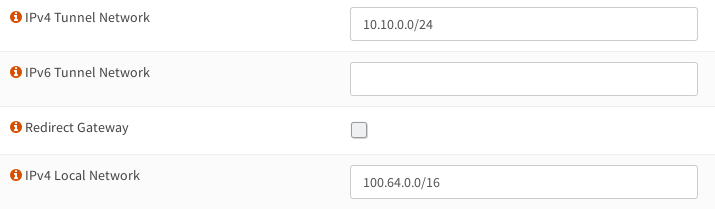
\includegraphics[width=\linewidth]{openvpn/settings-tunnel}
        \label{fig:openvpn-settings-tunnel}
    \end{figure}
    \vspace{-20pt}
    
    \subsection{Firewall rules}
    Firstly, it is necessary to allow incoming OpenVPN packets from the internet.
    To do so, create a new rule for interface WAN that accepts UDP packets with destination port 1194, the standard OpenVPN port.
    \begin{figure}[H]
        \centering
        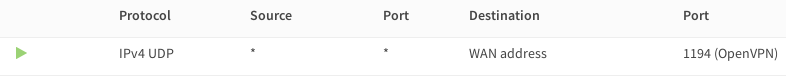
\includegraphics[width=\linewidth]{openvpn/rules-vpn}
        \label{fig:openvpn-rules-vpn}
    \end{figure}
    
    Then, allow access to \client and \ser networks for road warriors.
    Given that the specifics are not clear about the type of access the road warriors have and that they may have different needs than normal employees, allowing all TCP/UDP packets was considered a good compromise between security and functionality.
    
    In addition to creating the rules for the standard interfaces (those in \texttt{100.64.254.0/30}, \texttt{100.64.1.0/24} and \texttt{100.64.2.0/24}), we also define equivalent rules in the automatically-generated OpenVPN interface.
    \begin{figure}[H]
        \centering
        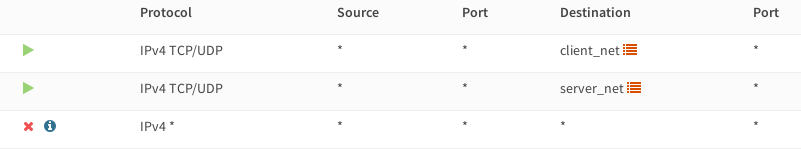
\includegraphics[width=\linewidth]{openvpn/rules-clients}
        \label{fig:rules-clients}
    \end{figure}
       
    \subsection{Clients}
    In VPN $\rightarrow$ OpenVPN $\rightarrow$ Client Export it is possible to download the OpenVPN configuration files.
    Obviously, it is necessary to insert the public IP for the WAN interface, which is usually fixed for enterprise networks.
    
    To start a new connection, execute the command \mintinline{sh}{openvpn --config FILE.ovpn} and insert a pair of valid credentials.
    \begin{figure}[H]
        \centering
        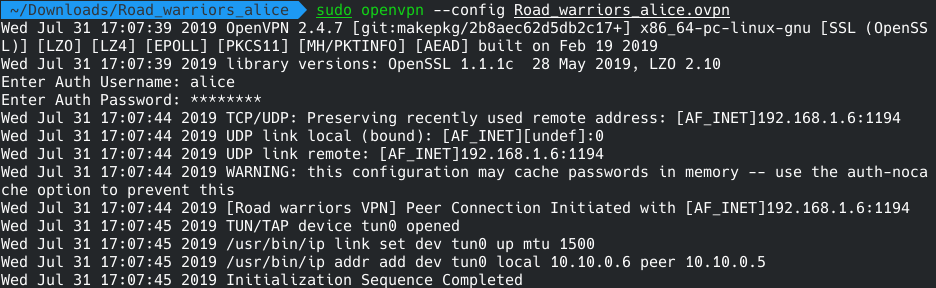
\includegraphics[width=\linewidth]{openvpn/client}
        \label{fig:openvpn-client}
    \end{figure}
    
    
    \section{VPN for the firewall tunnel}
    \fxnote{TODO}
    
    \section{Test of the configuration}
    \fxnote{TODO}
    
    \section{Final remarks}
    \fxnote{TODO}
\end{document}
